\chapter{Spezifikation der funktionellen Anforderungen}
\section{Produktbeschreibung}
TODO: Blablabla, alles wichtig und ganz toll

\section{Funktionelle Anforderungen}
\subsection{Umgebungsmodell}

\subsubsection{Ereignistabelle}
%wenn die Tabellen zu lang werden -> longtable
N = Nutzer, M = registriertes Mitglied, A = Administrator \\
M kann zusätzlich zu seinen, alle Ereignisse von N auslösen. A kann ebenso alle Ereignisse von M und N auslösen.

\begin{tabular}[ht]{|c|p{9.0em}|p{10.5em}|l|}
\hline
Nr & Ereignis & Datenfluß im System & Antwort des Systems \\
\hline\hline
1. & N sucht Buch & Suchbegriff & Suchtreffer \\\hline
2. & N wählt Buch & Buchnummer & Buchdaten Kommentare \\\hline
3. & N exportiert Buch & Exportanfrage &  BibTeX-Datei \\\hline
4. & M legt Buch an & Buchdaten & Bestätigung\_Buchanlegen \\\hline
5. & M ändert Buch & Buchdaten + Buchnummer & Bestätigung\_Buchändern\\\hline
6. & M löscht Buch & Buchnummer & Bestätigung\_Buchlöschen \\\hline
7. & M legt Kommentar an & Kommentardaten & Bestätigung\_Kommentaranlegen \\\hline
8. & M ändert Kommentar & Kommentardaten + Kommentarnumme & Bestätigung\_Kommentarändern \\\hline
9. & M löscht Kommentar & Kommentarnummer & Bestätigung\_Kommentarlöschen \\\hline
10.& M importiert BibTeX & BibTeX-Datei & Bestätigung\_BibTeXImport \\\hline
11.& A legt Mitglied an & Mitgliedsdaten & Bestätigung\_Mitgliedanlegen \\\hline
12.& A ändert Mitglied & Mitgliedsdaten + Mitgliedsnummer & Bestätigung\_Mitgliedändern \\\hline
13.& A löscht Mitglied & Mitgliedsnummer & Bestätigung\_Mitgliedlöschen \\\hline
14.& A ruft Mitglieder ab & - & Mitgliederliste \\\hline
\end{tabular}

\subsubsection{Kontextdiagramm}

%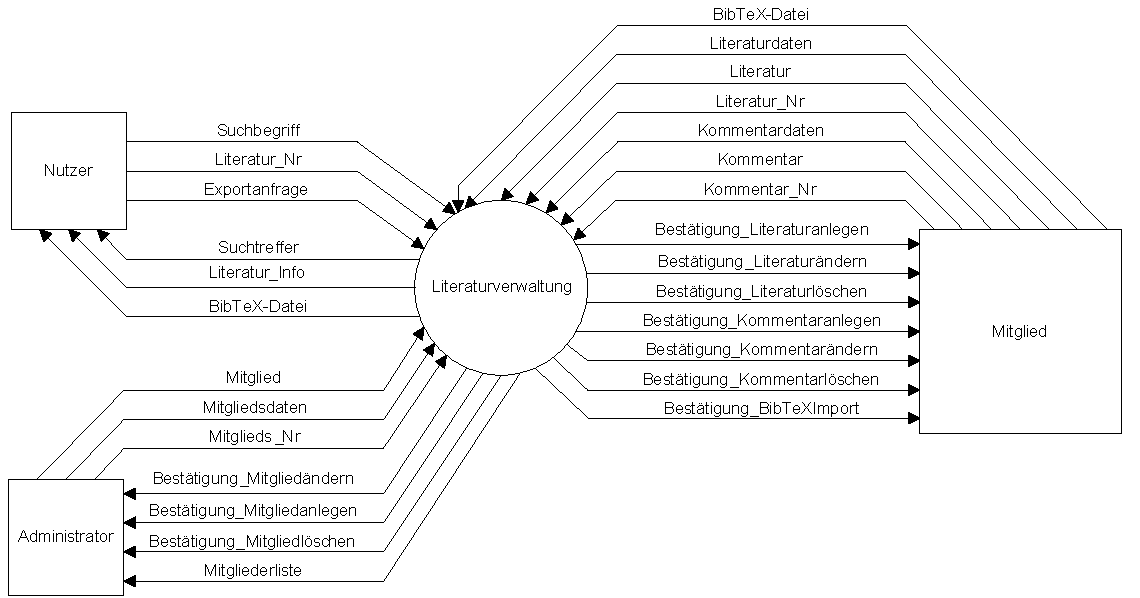
\includegraphics[scale=0.5]{kontextdiagramm}
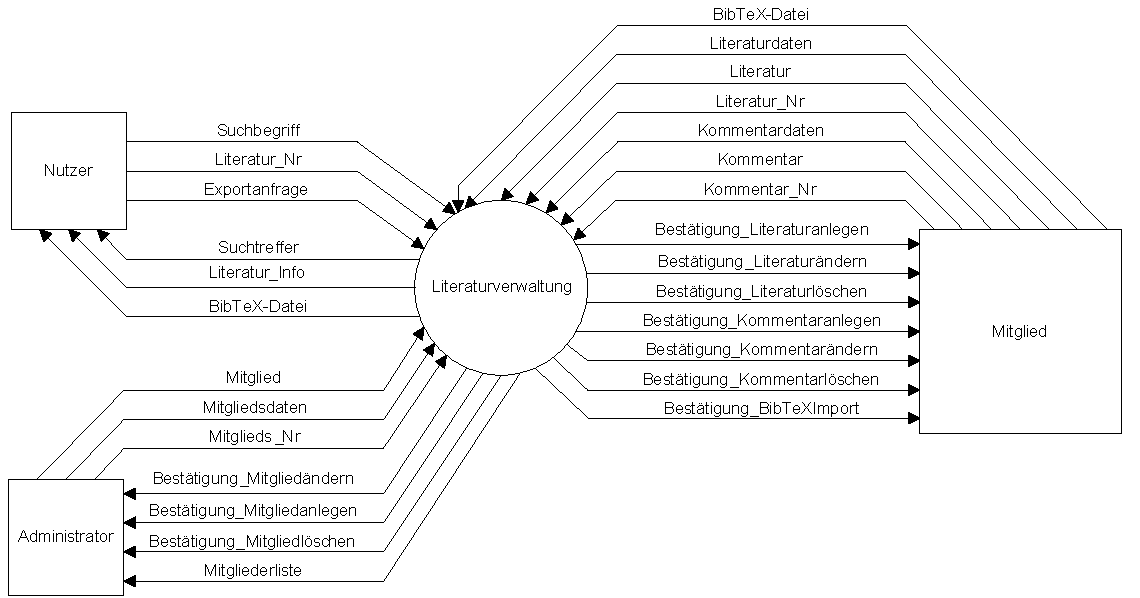
\includegraphics[scale=0.75]{kontextdiagramm}

\subsection{Verhaltensmodell}
\subsubsection{Grobes Verhaltensmodell (vergröbertes primäres Verhaltensmodell)}
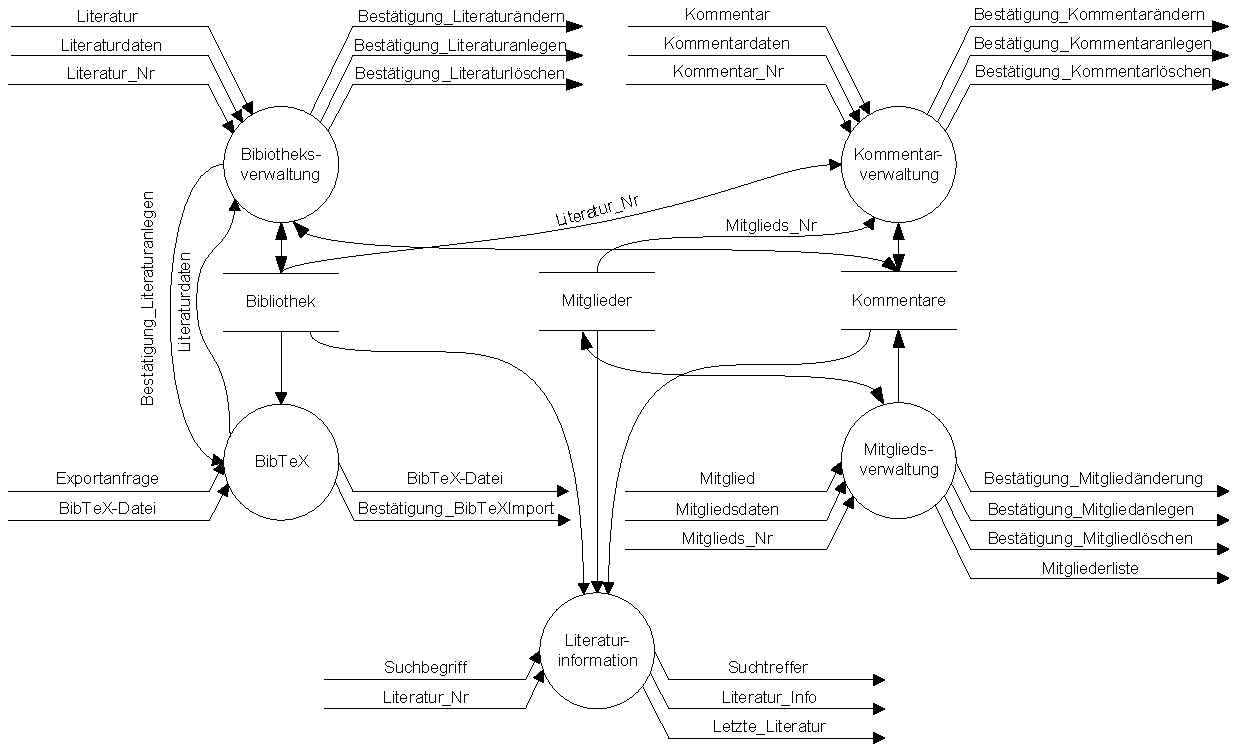
\includegraphics[scale=0.70]{grobes_verhaltensmodell}

\subsubsection{Primäres Verhaltensmodell}
\paragraph{Teilmodell BibTeX}
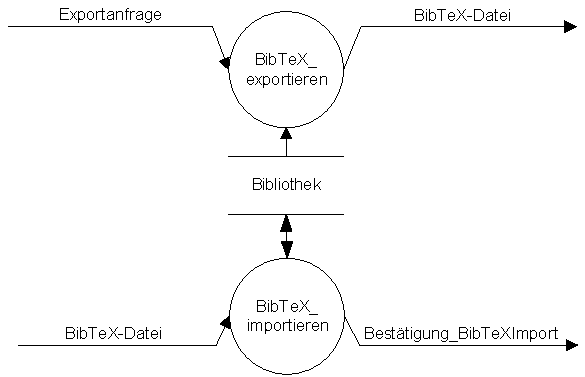
\includegraphics[scale=1.0]{teilmodell_bibtex}


\paragraph{Teilmodell Buchinformation}
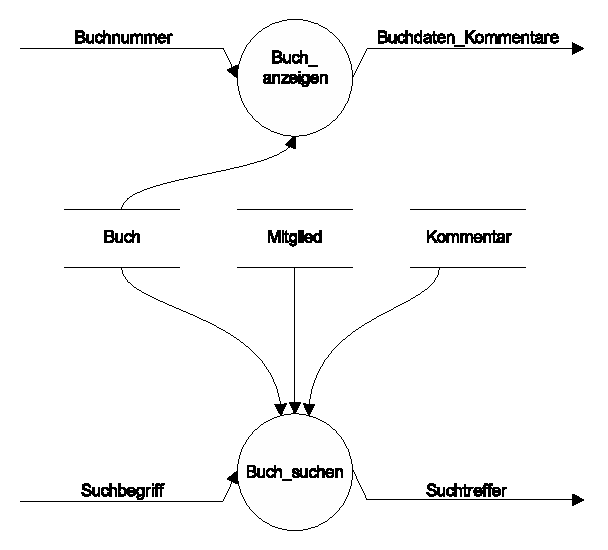
\includegraphics[scale=1.0]{teilmodell_buchinformation}

\paragraph{Teilmodell Buchverwaltung}
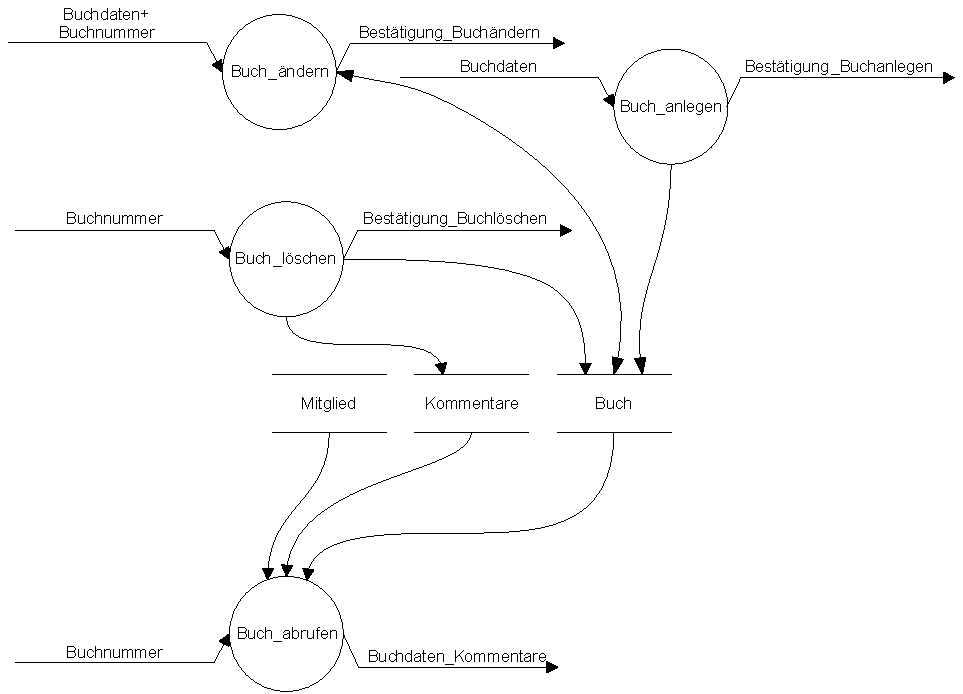
\includegraphics[scale=0.85]{teilmodell_buchverwaltung}

\paragraph{Teilmodell Kommentarverwaltung}
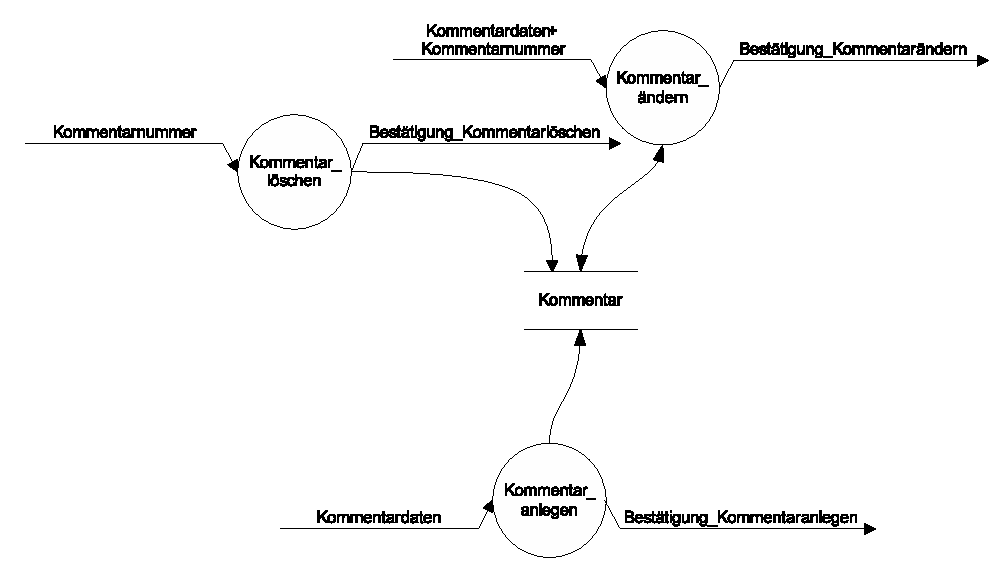
\includegraphics[scale=0.85]{teilmodell_kommentarverwaltung}

\paragraph{Teilmodell Mitgliederverwaltung}
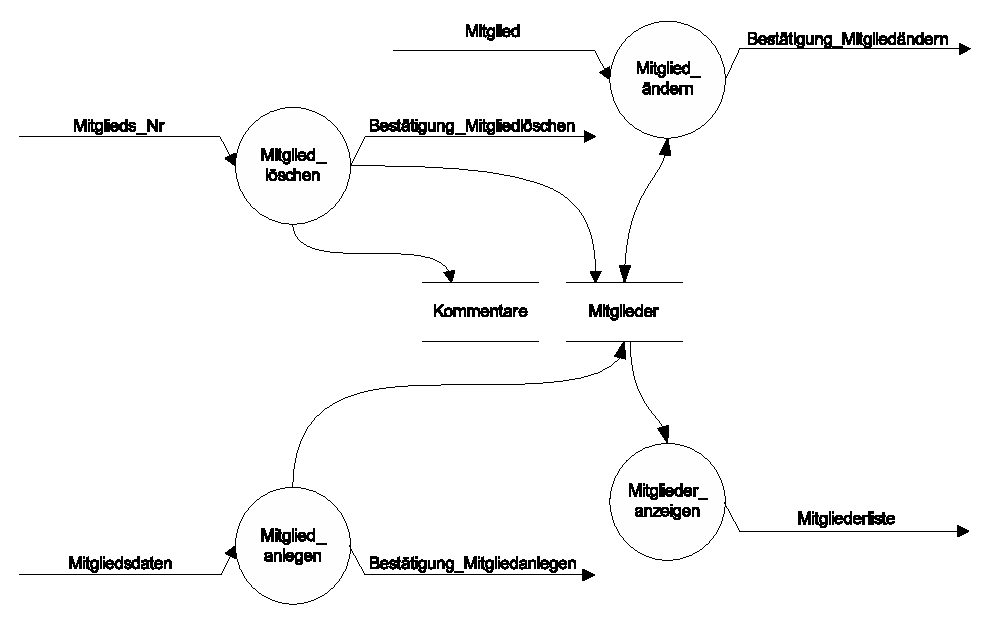
\includegraphics[scale=0.85]{teilmodell_mitgliederverwaltung}
\newpage

\subsubsection{Datenkatalog}
\begin{tabular}[ht]{|l|p{8.5cm}|}
\hline
Element & Strukturbeschreibung \\
\hline\hline
% Mitglieder
\emph{Benutzer} & \{Benutzer\} \\
\hline
Benutzer  & @Benutzer\_Nr + Name + Login + Passwort + Rechte \\
\hline
Benutzer\_Nr & gZahl *6stellig, 000001 $\leq$ Benutzer\_Nr $\leq$ 999999* \\ 
\hline
Name & <Vor>Name + <Nach>Name \\
\hline
Login & Zeichenkette12 \\
\hline
Passwort & Zeichenkette12 \\
\hline
Rechte & ["Benutzer" $\mid "$Administrator"] \\
\hline\hline

\emph{Literatur} & {Literatur} \\
\hline
Literatur & @Literatur\_Nr + Titel + Autor + ISBN + Jahr + Beschreibung + Ort + Stichworte \\
\hline
Literatur\_Nr & gZahl *6stellig, 000001 $\leq$ Literatur\_Nr $\leq$ 999999* \\
\hline
Titel & Zeichenkette40 \\
\hline
Autor & Zeichenkette40 \\
\hline
ISBN & gZahl *1stellig* + '-' + gZahl *4stellig* + '-' + gZahl *4stellig* + '-' + gZahl *1stellig* \\
\hline
Jahr & gZahl *4stellig* \\
\hline
Beschreibung & Zeichenkette250 \\
\hline
Ort & Zeichenkette40 \\
\hline
Stichworte & Zeichenkette100 \\
\hline\hline

\emph{Kommentar} & {Kommentar} \\
\hline
Kommentar & @Kommentar\_Nr + Kommentartext \\
\hline
Kommentarnummer & gZahl *6stellig, 000001 $\leq$ Kommentar\_Nr $\leq$ 999999* \\
\hline
Kommentartext & Zeichenkette400 \\
\hline\hline

Best\"atigung\_Benutzer\"anderung & Benutzer\_Nr + Zeichenkette "Ver\"anderung vorgenommen" \\
\hline
Best\"atigung\_Literatur\"anderung & Literatur\_Nr + Zeichenkette "Ver\"anderung vorgenommen" \\
\hline
Best\"atigung\_Kommentar\"anderung & Kommentar\_Nr + Zeichenkette "Ver\"anderung vorgenommen" \\
\hline
Literatur\_Info & Literatur\_Nr + Titel + Beschreibung + Kommentartext \\
\hline
Suchergebnis & Literatur\_Nr + Titel \\
\hline
BibTeX-Datei & *Datei im Bibtexformat* \\
\hline

\end{tabular}

\subsubsection{Beziehungen zwischen Speichern (ERD)}
%wenn die Tabellen zu lang werden -> longtable
TODO:
%\includegraphics[scale=0.5]{erd}

\subsubsection{Prozessspezifikation}
TODO: (siehe Beispielbeleg S. 9)

\paragraph{Prozess abc}

\paragraph{Prozess cde}

\subsection{Definition der Nutzerschnittstelle}
TODO (Generell, Fargestaltung)

\subsubsection{Ein- und Ausgabegeräte}
TODO Siehe Beispielbeleg S. 11

\paragraph{Legende zur Layoutdarstellung}
TODO Siehe Beispielbeleg S. 11

\paragraph{Grundfenster}
TODO

\paragraph{Menüs}
TODO

\paragraph{Fenster irgendwas}
TODO
